\documentclass{ximera}

%% Where to look for inputs
\makeatletter     %% make "@" a letter-character
\def\input@path{  %% When looking for files,
{./}              %% look first at your level
{./coverArt/}     %% then in this folder,
{./introduction/} %% then in this folder,
}
\makeatother      %% make "@" an other-character

%% Where to find images
\graphicspath{                      %% When looking for images, 
{./}                                %% look first at your level,
{./setup/}                          %% then in this folder,
{./graphicsVideosAndInteractives/}  %% then in this folder,
}



% Custom Commands


%% These may change and should be checked! 
\newcommand{\docURL}{\url{https://github.com/ximeraProject/ximeraFirstSteps/ximeraUserManual}}
\newcommand{\testURL}{\url{https://github.com/ximeraProject/tests}}
\newcommand{\experimentalURL}{\url{https://github.com/ximeraProject/experimental}}
\newcommand{\xfsURL}{https://go.osu.edu/xfs}
\newcommand{\xfgURL}{https://go.osu.edu/ximera-flash-grant}

\newcommand{\event}[1]{\def\theevent{#1}}
\newcommand{\theevent}{}


\newif\ifcolor %% for color cover
\colorfalse
\colorlet{bkgndcr}{white}
\colorlet{txtcr}{black}
\colorlet{otherbkgndcr}{white}
\colorlet{othertxtcr}{black}


\usepackage{qrcode} %% For QR Codes
\usepackage[normalem]{ulem} % for strikeout
\usepackage{multicol} % multicols -- PDF only

\makeatletter
%% Make Front style
\newcommand\frontstyle{%
  \def\activitystyle{activity-chapter}
  \def\maketitle{%
                {\flushleft\small\sffamily\bfseries\@pretitle\par\vspace{-1.5em}}%
                {\flushleft\LARGE\sffamily\bfseries\@title \par }%3
                {\vskip .6em\noindent\textit\theabstract\setcounter{problem}{0}\setcounter{section}{0}}%
                \par\vspace{2em}    
                \phantomsection\addcontentsline{toc}{section}{\textbf{\@title}}%
                \setcounter{titlenumber}{0}
}}

\renewcommand\chapterstyle{%
  \def\activitystyle{activity-chapter}
  \normalsize
  %\onecolumn
  \def\maketitle{%
    \addtocounter{titlenumber}{1}%
                    {\flushleft\small\sffamily\bfseries\@pretitle\par\vspace{-1.5em}}%
                    {\flushleft\LARGE\sffamily\bfseries\thetitlenumber\hspace{1em}\@title \par }%
                    {\vskip .6em\noindent\textit\theabstract\setcounter{problem}{0}\setcounter{section}{0}}%
                    \par\vspace{2em}
                    \phantomsection\addcontentsline{toc}{section}{\textbf{\thetitlenumber\hspace{1em}\@title}}%
}}

%% Redefine section and subsection
\renewcommand\section{\@startsection {section}{1}{\z@}%
                                   {-3.5ex \@plus -1ex \@minus -.2ex}%
                                   {2.3ex \@plus.2ex}%
                                   {\boldmath\normalfont\large\bfseries\sffamily}}
\renewcommand\subsection{\@startsection{subsection}{2}{\z@}%
                                     {-3.25ex \@plus -1ex \@minus -.2ex}%
                                     {1.5ex \@plus .2ex}%
                                     {\boldmath\normalfont\large\bfseries\sffamily}}


\renewcommand\paragraph{\@startsection{paragraph}{4}{\z@}%
                                    {3.25ex \@plus1ex \@minus.2ex}%
                                    {-1em}%
                                    {\boldmath\normalfont\normalsize\bfseries\sffamily}}
\makeatother

\title{Exercise banks}
\author{Bart Snapp}

\begin{document}
\begin{abstract}
  Ximera can present exercise banks.
\end{abstract}
\maketitle


% \section{Exercise banks}

Exercise banks can be made with \verb!xourse! files. If you are making an
exercise bank, you might want to have essentially one exercise per file.

\paragraph{File structure}

\begin{center}
  \scalebox{.7}{
    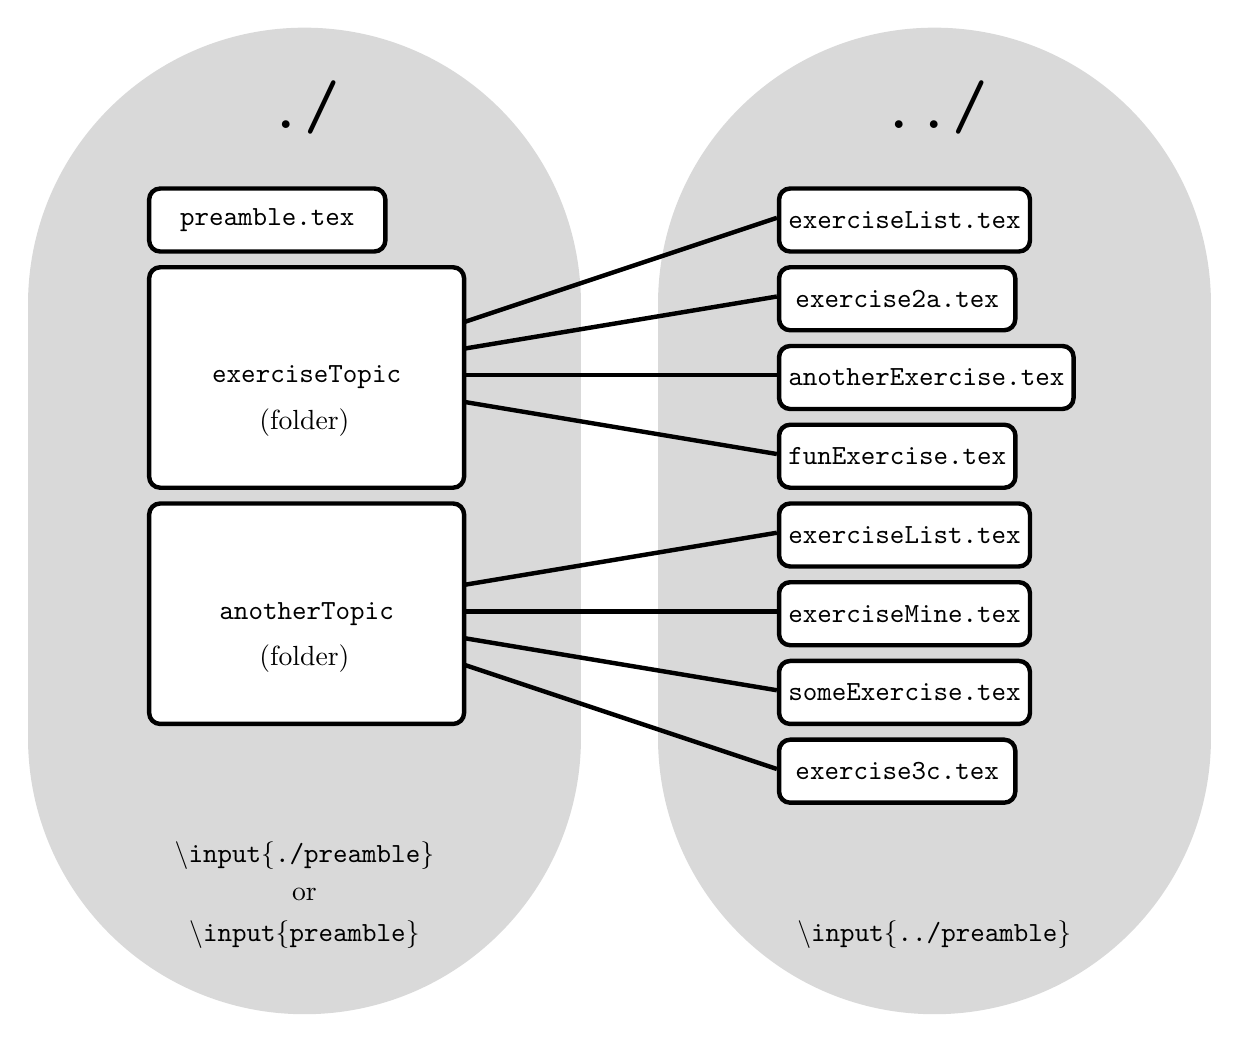
\begin{tikzpicture}
      % Define styles for nodes
      \tikzstyle{document} = [anchor=north west,draw, rounded corners,
      rectangle,
      minimum width=3cm,fill=white, minimum height=.8cm, ultra
      thick,font=\ttfamily]
      \tikzstyle{folder} = [anchor=north west,draw, rectangle, rounded corners,
      minimum width=4cm,fill=white, minimum height=2.8cm, ultra
      thick,font=\ttfamily]

      % Thick grey lines
      \draw[line width=200pt,white!85!black,line cap=round] (2,1.5) -- (2,-4);
      \draw[line width=200pt,white!85!black,line cap=round] (10,1.5) --
      (10,-4);

      % Connections
      \draw[ultra thick] (2,.6) -- (8,2.6);
      \draw[ultra thick] (2,.6) -- (8,1.6);
      \draw[ultra thick] (2,.6) -- (8,.6);
      \draw[ultra thick] (2,.6) -- (8,-.4);

      \draw[ultra thick] (2,-2.4) -- (8,-1.4);
      \draw[ultra thick] (2,-2.4) -- (8,-2.4);
      \draw[ultra thick] (2,-2.4) -- (8,-3.4);
      \draw[ultra thick] (2,-2.4) -- (8,-4.4);

      % Symbols at top
      \node at (2,4) {\Huge \tt ./};
      \node at (10,4) {\Huge \tt ../};

      % Define the folders at top level
      \node[document] at (0,3) {preamble.tex};
      \node[folder] at (0,2) {exerciseTopic};
      \node[] at (2,0) {(folder)};
      \node[folder] at (0,-1) {anotherTopic};
      \node[] at (2,-3) {(folder)};

      % Define the documents in the exercises folder
      \node[document] at (8,3) {exerciseList.tex};
      \node[document] at (8,2) {exercise2a.tex};
      \node[document] at (8,1) {anotherExercise.tex};
      \node[document] at (8,0) {funExercise.tex};

      \node[document] at (8,-1) {exerciseList.tex};
      \node[document] at (8,-2) {exerciseMine.tex};
      \node[document] at (8,-3) {someExercise.tex};
      \node[document] at (8,-4) {exercise3c.tex};

      % paths at bottom
      \node at (2,-5.5) {\tt\textbackslash input\{./preamble\}};
      \node at (2,-6) {or};
      \node at (2,-6.5) {\tt\textbackslash input\{preamble\}};
      \node at (10,-6.5) {\tt\textbackslash input\{../preamble\}};
    \end{tikzpicture}
  }
\end{center}

The individual exercises that live in folders might look something like:

\begin{verbatim}
\documentclass{ximera}
\begin{document}
\begin{exercise}
Compute:
\[
  \frac{\partial}{\partial x} \sin(3xyx) 
  = \answer{3yz\cos(3xyz)}
\]
\end{exercise}
\end{document}
\end{verbatim}

In this case, the \verb!exerciseList! within \verb!exerciseTOpic! might look
like

\begin{verbatim}
\documentclass{xourse}
%% Where to look for inputs
\makeatletter     %% make "@" a letter-character
\def\input@path{  %% When looking for files,
{./}              %% look first at your level
{./coverArt/}     %% then in this folder,
{./introduction/} %% then in this folder,
}
\makeatother      %% make "@" an other-character

%% Where to find images
\graphicspath{                      %% When looking for images, 
{./}                                %% look first at your level,
{./setup/}                          %% then in this folder,
{./graphicsVideosAndInteractives/}  %% then in this folder,
}



% Custom Commands


%% These may change and should be checked! 
\newcommand{\docURL}{\url{https://github.com/ximeraProject/ximeraFirstSteps/ximeraUserManual}}
\newcommand{\testURL}{\url{https://github.com/ximeraProject/tests}}
\newcommand{\experimentalURL}{\url{https://github.com/ximeraProject/experimental}}
\newcommand{\xfsURL}{https://go.osu.edu/xfs}
\newcommand{\xfgURL}{https://go.osu.edu/ximera-flash-grant}

\newcommand{\event}[1]{\def\theevent{#1}}
\newcommand{\theevent}{}


\newif\ifcolor %% for color cover
\colorfalse
\colorlet{bkgndcr}{white}
\colorlet{txtcr}{black}
\colorlet{otherbkgndcr}{white}
\colorlet{othertxtcr}{black}


\usepackage{qrcode} %% For QR Codes
\usepackage[normalem]{ulem} % for strikeout
\usepackage{multicol} % multicols -- PDF only

\makeatletter
%% Make Front style
\newcommand\frontstyle{%
  \def\activitystyle{activity-chapter}
  \def\maketitle{%
                {\flushleft\small\sffamily\bfseries\@pretitle\par\vspace{-1.5em}}%
                {\flushleft\LARGE\sffamily\bfseries\@title \par }%3
                {\vskip .6em\noindent\textit\theabstract\setcounter{problem}{0}\setcounter{section}{0}}%
                \par\vspace{2em}    
                \phantomsection\addcontentsline{toc}{section}{\textbf{\@title}}%
                \setcounter{titlenumber}{0}
}}

\renewcommand\chapterstyle{%
  \def\activitystyle{activity-chapter}
  \normalsize
  %\onecolumn
  \def\maketitle{%
    \addtocounter{titlenumber}{1}%
                    {\flushleft\small\sffamily\bfseries\@pretitle\par\vspace{-1.5em}}%
                    {\flushleft\LARGE\sffamily\bfseries\thetitlenumber\hspace{1em}\@title \par }%
                    {\vskip .6em\noindent\textit\theabstract\setcounter{problem}{0}\setcounter{section}{0}}%
                    \par\vspace{2em}
                    \phantomsection\addcontentsline{toc}{section}{\textbf{\thetitlenumber\hspace{1em}\@title}}%
}}

%% Redefine section and subsection
\renewcommand\section{\@startsection {section}{1}{\z@}%
                                   {-3.5ex \@plus -1ex \@minus -.2ex}%
                                   {2.3ex \@plus.2ex}%
                                   {\boldmath\normalfont\large\bfseries\sffamily}}
\renewcommand\subsection{\@startsection{subsection}{2}{\z@}%
                                     {-3.25ex \@plus -1ex \@minus -.2ex}%
                                     {1.5ex \@plus .2ex}%
                                     {\boldmath\normalfont\large\bfseries\sffamily}}


\renewcommand\paragraph{\@startsection{paragraph}{4}{\z@}%
                                    {3.25ex \@plus1ex \@minus.2ex}%
                                    {-1em}%
                                    {\boldmath\normalfont\normalsize\bfseries\sffamily}}
\makeatother
\title{My exercise banks}
\begin{document}
\begin{abstract}
Here is an exercise bank
\end{abstract}
\maketitle

\practice{exercise2a}
\practice{anotherExercise}
\practice{funExercise}

\end{document}
\end{verbatim}
IF you don't give your \verb!xourse! file a title, it will not show up on the
front page.
Instead you can link directly to the file by going to something like:
\begin{center}
  \verb!https://some.ximera.server/DEPOLOY-NAME/exerciseTopic/exerciseList!
\end{center}

\paragraph{Exercises as part of a course} can be included as a folder within
the section that the exercises address. The next section will address this in
detail.



\end{document}